\chapter{Grundlagen}
In diesem Kapitel sollen die für das weitere Verständnis notwendigen theoretischen Grundlagen erläutert werden. Dazu gehört zunächst der Aufbau des Netzwerks in einem Fahrzeug. Des Weiteren werden relevante Grundlagen der Cyber Security erklärt.

\section{Automotive Networking}
Im Inneren von Autos befinden sich heutzutage eine Vielzahl elektronischer Systeme, von denen jedes mit benachbarten Komponenten kommunizieren kann. Die einzelnen elektronischen Systeme werden als \acp{ECU} bezeichnet. Moderne Autos enthalten in der Regel über 50 verschiedene \acsp{ECU} \cite[vgl.][6]{Miller.2013}. Da diese Kontrolleinheiten zum Teil lebensentscheidende Aufgaben übernehmen, muss die Kommunikation zwischen den Einheiten möglichst in Echtzeit erfolgen. \\

\begin{figure}[H]
\centering
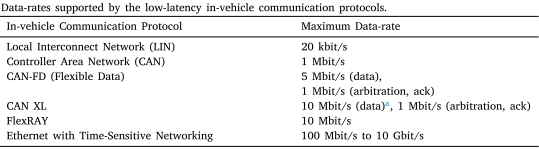
\includegraphics[width=\textwidth]{communication-protocols}
\label{fig:communication-protocols}
\caption{Verschiedene Kommunikationsprotokolle in Automobil-Netzwerken}
\quelle{\cite[2]{MohammadAshjaei.2021}}
\end{figure}

Für die Vernetzung der \acsp{ECU} kommen verschiedene Technologien zum Einsatz (siehe Abbildung \ref{fig:communication-protocols}). Die relevantesten davon werden im Folgenden genauer erläutert. Die wichtigste  davon ist im Automotive-Bereich der sogenannte \acs{CAN}-Standard.

\subsection{Controller Area Network}
Die elektronischen Kontrolleinheiten eines Autos sind typischerweise über einen oder mehrere Busse, die auf dem \ac{CAN}-Standard basieren, miteinander verbunden. Hierbei kommunizieren die \acsp{ECU} über \acs{CAN}-Pakete. Diese werden an alle Komponenten gesendet, welche dann jeweils basierend auf dem Inhalt entscheiden, ob das Paket für sie bestimmt ist oder nicht. Eine Identifikation der Quelle oder Authentisierung gibt es in diesem Standard nicht. \cite[vgl.][7]{Miller.2013} \\
Generell wird meistens zwischen High Speed \acs{CAN} und Low Speed \acs{CAN} unterschieden. High Speed \acs{CAN} wird eingesetzt, wenn bei der Übertragung hohe Geschwindigkeit benötigt wird, beispielsweise bei sicherheitskritischen Anwendungsfällen. Außerdem wird bietet sich die Verwendung von High Speed \acs{CAN} bei der Übertragung von großen Datenmengen an.
In Abbildung \ref{fig:canbus-ford2010} ist das \acs{CAN}-Netzwerk eines 2010 Ford Escape dargestellt. Das abgebildete Netzwerk verfügt über zwei Busse, einen medium speed (MS) und einen high speed (HS) \acs{CAN}-Bus. Beide Busse enden hier im \ac{DLC} (siehe Kapitel \ref{OBD-II}).
In Automotive Netzwerken lassen sich zwei Arten von \acs{CAN}-Paketen finden: normale \acs{CAN}-Pakete und diagnostische \acs{CAN}-Pakete. 

\begin{figure}[H]
\centering
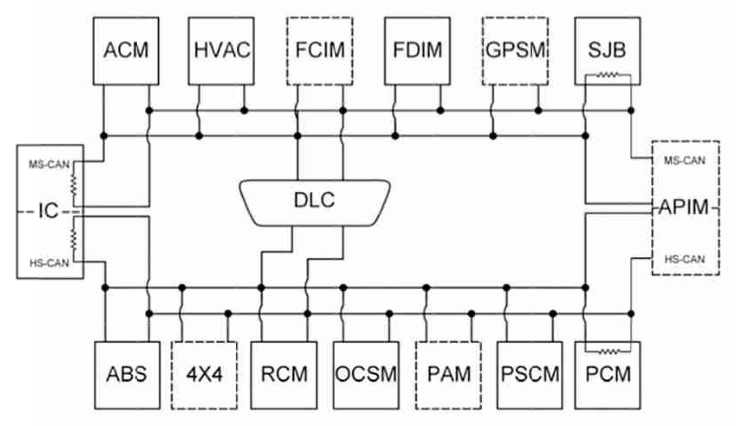
\includegraphics[width=\textwidth]{Miller_canbus-ford2010}
\label{fig:canbus-ford2010}
\caption{Beispiel des \acs{CAN}-Netzwerks eines 2010 Ford Escape}
\quelle{\cite[19]{Miller.2013}}
\end{figure}

\subsubsection{Normale \acs{CAN}-Pakete}
Normale Pakete werden von \acsp{ECU} gesendet und können entweder Informationen oder Befehle enthalten. Typischerweise werden sie alle Millisekunden gesendet. Auf Anwendungsebene enthalten die \acs{CAN}-Pakete einen Identifier, die zu übertragenden Daten und manchmal noch eine Prüfsumme, um sicherzustellen, dass das Paket korrekt übertragen wurde. Der Identifier gibt sowohl an, für welche \acsp{ECU} das Paket bestimmt ist, als auch, welche Priorität das Paket hat. \cite[vgl.][9]{Miller.2013}\\
Das Format einer \acs{CAN}-Botschaft ist in Abbildung \ref{fig:CanBotschaft} dargestellt. Es besteht aus folgenden Bestandteilen:
\subparagraph{Header} CAN ist ein Broadcast-System, bei dem jeder Sender seine Botschaften mit einem eindeutigen Message Identifier markiert.
\subparagraph{Message Identifier} Der Message Identifier kennzeichnet eine Botschaft und dient zur eindeutigen Identifizierung. Er kann entweder 11 Bit (CAN 2.0A) oder 29 Bit (CAN 2.0B) lang sein und enthält zusätzlich 1 bis 3 Steuerbits.
\subparagraph{Control Bits} Die Steuerbits im Control-Feld umfassen den Data Length Code (DLC), der die Anzahl der übertragenen Nutzdatenbytes angibt, sowie eine 15-Bit-Prüfsumme, auch genannt Cyclic Redundancy Check (CRC) zur Fehlererkennung.
\subparagraph{Payload} Die Nutzdaten (Payload) einer Botschaft können zwischen 0 und 8 Datenbytes umfassen.
\subparagraph{Acknowledge und End of Frame} Die CAN-Controller der Empfänger senden eine positive Empfangsbestätigung oder eine Fehlermeldung (Error Frame) innerhalb des Acknowledge und End of Frame Felds.
\subparagraph{Stuffing Bits} Stuffing Bits werden verwendet, um den Bittaktgenerator von Empfängern zu synchronisieren. Sie werden eingefügt, um sicherzustellen, dass nicht mehr als fünf aufeinanderfolgende Bits denselben Wert haben. \cite[61\psqq]{Zimmermann.2014}

\begin{figure}[h]
\centering
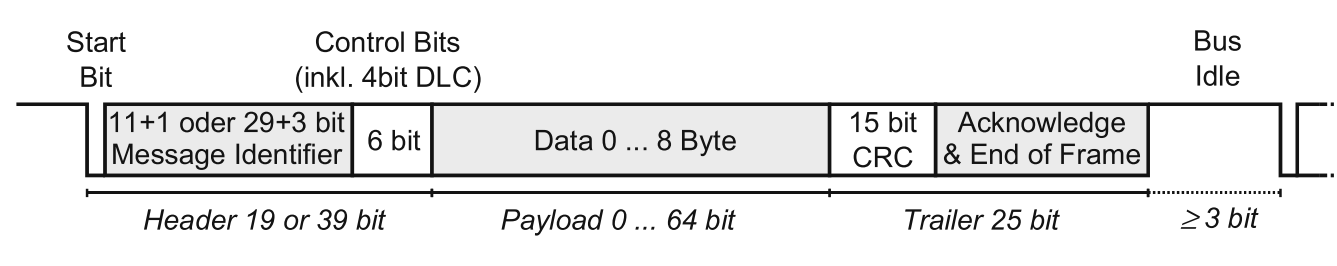
\includegraphics[width=\textwidth]{Zimmermann_CanBotschaft}
\label{fig:CanBotschaft}
\caption{Format einer \acs{CAN}-Botschaft}
\quelle{\cite[61]{Zimmermann.2014}}
\end{figure}


\subsubsection{Diagnostische \acs{CAN}-Pakete}
Diagnostische Pakete tauchen während des normalen Betriebs des Autos im Normalfall nicht auf. Sie werden von Diagnose-Werkzeugen gesendet, die beispielsweise von Mechanikern genutzt werden um mit den \acsp{ECU} im Auto zu kommunizieren. So können Mängel und Fehlfunktionen entdeckt oder andere Informationen gewonnen werden. Das Format von diagnostischen \acs{CAN}-Paketen ähnelt dem von normalen Paketen, erfolgt jedoch meist nach strengeren Konventionen. Standards hierfür sind zum Beispiel ISO-TP, ISO 14229 und ISO 14230. \cite[vgl.][10]{Miller.2013}

\subsection{Local Interconnect Network}
Ein weiteres relevantes Protokoll im Automotive Bereich ist das \ac{LIN} Protokoll. Es wurde 1998 in Zusammenarbeit von Audi, BMW, DaimlerChrysler, Volvo, Volkswagen, VCT und Motorola entwickelt mit dem Ziel, ein möglichst kosteneffizientes Kommunikationsprotokoll zu schaffen \cite[57]{Fijalkowski.2011}.
Das \acs{LIN}-Protokoll basiert auf dem Serial Connections Interface Datenformat und ist in einer Single Master/Multiple Slaves Architektur aufgebaut. Das bedeutet, dass eine elektronische Kontrolleinheit als Masterknoten fungiert und andere elektronische Slave-Einheiten miteinander verbindet.
%Genauere Funktionsweise / Paketaufbau ergänzen

\subsubsection{Aufbau}
Nachrichtenpakete bestehen im \acs{LIN}-Standard aus einem Header und einem Data Frame. Der Header enthält einen Synchronisation Break, ein Synchronisation Byte und einen Message Identifier. Die ersten beiden Bestandteile sind für die Nachrichtensynchronisierung notwendig. Der Identifier wird benötigt, damit Knoten erkennen können, ob eine Nachricht für sie bestimmt ist. Der Data Frame ist nach dem 8N1-Schema aufgebaut. Das bedeutet, dass jedes Paket ein Startbit, acht Datenbits, kein Paritätsbit und ein Stopbit besitzt. \cite[58]{Fijalkowski.2011} \\
Im \acs{LIN}-Standard sind drei Arten von Kommunikation erlaubt.
\begin{enumerate}
\item Master to Slave, beziehungsweise Master to Multiple Slaves
\item Slave to Master
\item Slave to Slave
\end{enumerate}
Die Slaves können somit auch untereinander ohne Beiteiligung des Masters kommunizieren. \cite[59]{Fijalkowski.2011}

\subsubsection{Anwendung}
\ac{LIN} zeichnet sich wie oben erwähnt vor allem durch seine Kosteneffizienz aus. Allerdings bietet das Protokoll deutlich weniger Bandbreite als \acs{CAN}. Somit wird es vor allem an Stellen im Fahrzeug eingesetzt, wo nicht viel Bandbreite notwendig ist. Beispielsweise wird \acs{LIN} häufig für die Steuerung von Türen, Dach, Sitzen und dem Lenkrad verwendet. \cite[59]{Fijalkowski.2011} \\
Für den Aufbau eines Netzwerks mit den zwei Protokollen gibt es zwei gängige Ansätze:
\begin{enumerate}
\item Mehrere \acsp{ECU} werden über \acs{LIN} mit einer zentralen \acs{ECU} verbunden. Die Verbindung dieser zentralen \acsp{ECU} erfolgt mit dem \acs{CAN}-Standard.
\item Alle \acsp{ECU} werden über \acs{LIN} mit einer zentralen \acs{ECU} verbunden.
\end{enumerate}
Der zweite Ansatz ist skalierbarer, da ohne großen Aufwand neue Knoten hinzugefügt werden können. Der erste Ansatz ermöglicht jedoch eine deutlich höhere Bandbreite bei der Kommunikation zwischen den Einheiten. \cite[58]{Fijalkowski.2011}


\subsection{FlexRay}
Der \ac{CAN} Standard weist neben seinen Stärken auch einige Schwächen auf. Beispielsweise ist die realistisch erreichbare Datenrate beschränkt, zudem lassen sich sehr hohe Datenraten nur mit kurzen Stichverbindungen erreichen. Außerdem verfügt das System nur über einen Kanal und versagt somit bei Ausfall der Busverbindung. Aus diesen Gründen hielten viele Fachleute eine Neuentwicklung für notwendig und sinnvoll \cite[96]{Zimmermann.2014}. Daher wurde FlexRay als Ersatz für \acs{CAN} entwickelt. In der Praxis wird es allerdings größtenteils mehr als Ergänzung als als vollständiger Ersatz eingesetzt \cite[97]{Zimmermann.2014}. Dies könnte an den höheren Kosten aufgrund größerer Komplexität von FlexRay liegen.s FlexRay ermöglicht Aufbauten in Linien- und Sterntopologien. Diese können einkanalig oder zweikanalig sein.\\
Der Aufbau einer FlexRay-Botschaft ist in Abbildung \ref{fig:FlexRayBotschaft} veranschaulicht. Zu Beginn einer FlexRay-Botschaft stehen 5 Steuerbits, in denen Sonderinformationen über die Nachricht angezeigt werden können. Anschließend folgen die Frame ID mit dem Zeitslot der Botschaft, die Nutzdatenlänge, eine Cyclic-Redundancy-Check-Prüfsumme und ein Zykluszähler. 


\begin{figure}[H]
\centering
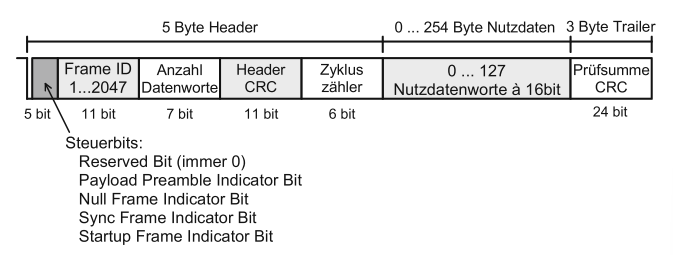
\includegraphics[width=\textwidth]{Zimmermann_FlexrayBotschaft}
\label{fig:FlexRayBotschaft}
\caption{Aufbau einer FlexRay-Botschaft}
\quelle{\cite[101]{Zimmermann.2014}}
\end{figure}


\subsection{Media Oriented System Transport}
Das \ac{MOST} Protokoll wird vor allem in Infotainment-Systemen von Autos eingesetzt. Anstelle von Kabeln werden hier Lichtwellenleiter verwendet. Somit ist das Signal unempfänglich gegenüber elektromagnetischer Einstrahlung. Es wird unterschieden zwischen \acs{MOST}25, \acs{MOST}50 und \acs{MOST}150, welche sich in Paketgröße und Bandbreite unterscheiden. Ein \acs{MOST}-Netzwerk ist meist als Ringtopologie aufgebaut (vergleiche Abbildung \ref{fig:MOST-NetworkMasterSlave}). Auch im \acs{MOST}-Protokoll gibt es Master- und Slave-Knoten. Der Master-Knoten ist häufig ein Gateway zu einem \acs{CAN}-Bus.\\

\begin{figure}[H]
\centering
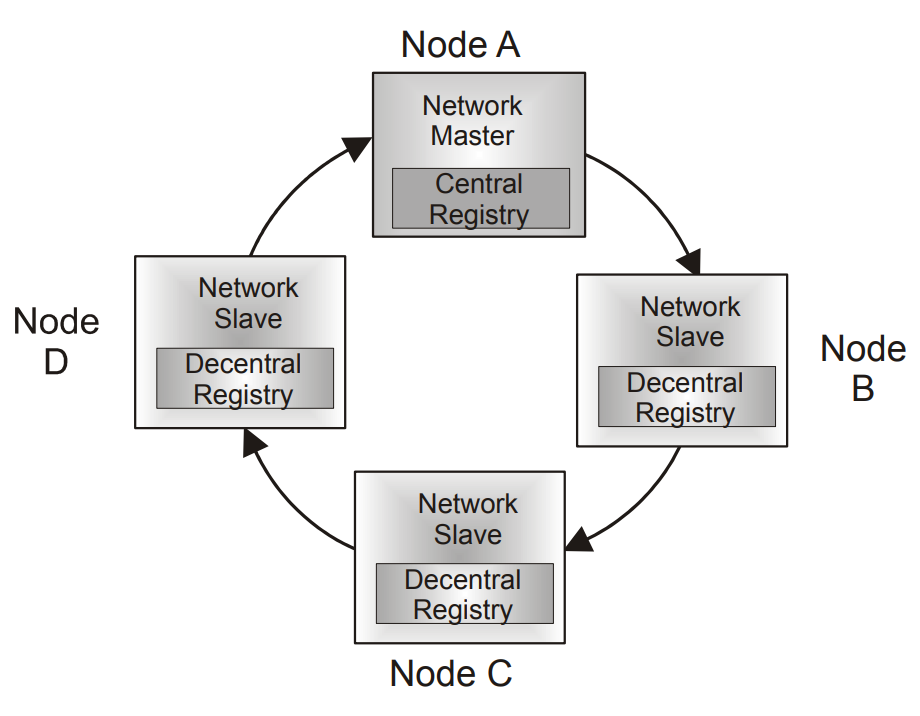
\includegraphics[width=\textwidth]{Grzemba_MOST_NetworkMasterSlave}
\label{fig:MOST-NetworkMasterSlave}
\caption{Ringtopologie eines \acs{MOST}-Bus}
\quelle{\cite[40]{Grzemba.2007}}
\end{figure}

\subsubsection{Paketaufbau}
Der Aufbau eines \acs{MOST}25-Pakets ist in Abbildung \ref{fig:MOST-frame} dargestellt. Es folgt eine kurze Erklärung der Einzelnen Bestandteile.
\subparagraph{Anfangsfeld (Preamble)} Das Anfangsfeld wird vom TimingMaster generiert und dient der Synchronisation der Slaves.
\subparagraph{Abgrenzungsfeld (Boundary Descriptor)}Das Abgrenzungsfeld definiert die in Vier-Byte-Schritten verschiebbare Grenze zwischen Stream- und Paketdaten.
\subparagraph{Datenfeld (stream data, packet data)}Das Datenfeld besteht aus 60 Bytes die nach Bedarf zwischen Streamdaten und Paketdaten aufgeteilt werden können.
\subparagraph{Kontrollbytes (Frame Control)}Die Kontrollbytes am Ende dienen der Kontrolle des Frames.
\subparagraph{Paritätsfeld (Parity Bit)}Das Paritätsfeld ermöglicht das Erkennen von Bit-Fehlern im Frame.
\\

\begin{figure}[H]
\centering
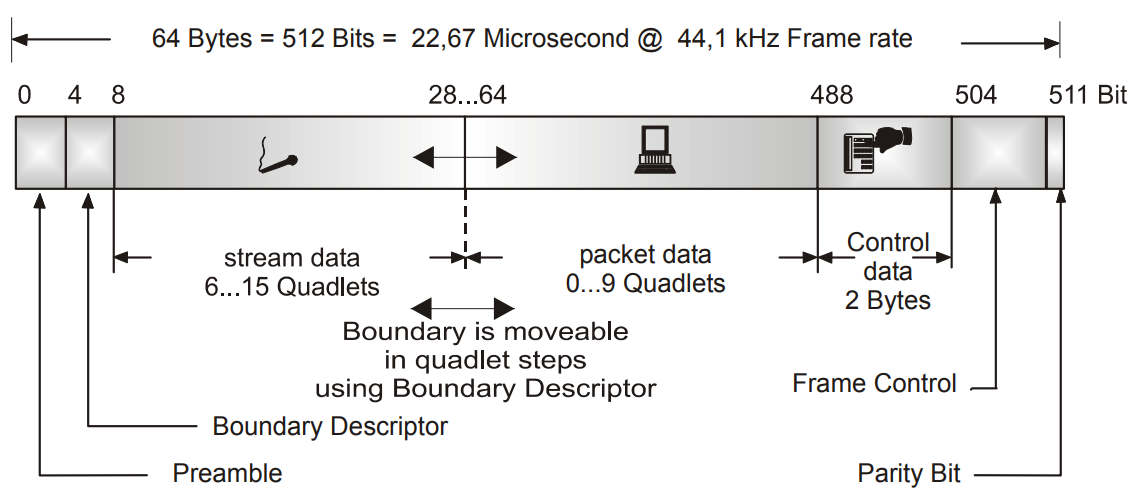
\includegraphics[width=\textwidth]{Grzemba_MOST_frame}
\label{fig:MOST-frame}
\caption{Aufbau eines \acs{MOST}25-Pakets}
\quelle{\cite[88]{Grzemba.2007}}
\end{figure}


\subsection{Automotive Ethernet}
Die Vielzahl inkompatibler und nur in der Automobilindustrie verwendeter Lösungen resultierte in hohen Kosten und kontinuierlichem Weiterentwicklungsaufwand. Zudem steigt der Bandbreitenbedarf. Daher wird das im Bürobereich etablierte Konzept Ethernet/IP relevanter für den Automobilbereich. \cite[138]{Zimmermann.2014}\\
Die in diesem Standard verwendeten Protokolle \ac{IP}, \ac{TCP} und \ac{UDP} werden außerdem bereits von den meisten computerähnlichen Geräten unterstützt. Das ermöglicht eine transparente Kommunikation und vereinfacht die Integration von Consumergeräten erheblich \cite{Zimmermann.2014}. Ethernet war ursprünglich ein Linienbussystem, wird heutzutage aber meistens als Sterntopologie mit Switches an Kopplungspunkten umgesetzt. \\
In Abbildung \ref{fig:EthernetPaket} ist der Aufbau eines Ethernet-Pakets dargestellt. 
Die Präambel und der Start Frame Delimiter spielen eine Rolle bei der Taktsynchronisation bei manchen Physical Layern. Die Ziel- und Quell-MAC-Adresse dienen der Geräteadressierung. Das VLAN-Tag erlaubt die Bildung von Unternetzen. Das Typfeld kennzeichnet den Typ des Inhalts des darauf folgenden Datenfelds. Das Datenfeld enthält den eigentlichen Nachrichteninhalt. Am Ende jedes Pakets befindet sich noch die Frame Check Sequence zur Detektion von Übertragungsfehlern. Beim Eintritt eines Übertragungsfehlers wird die Botschaft automatisch vom Empfänger verworfen. \cite[140]{Zimmermann.2014}\\

\begin{figure}[H]
\centering
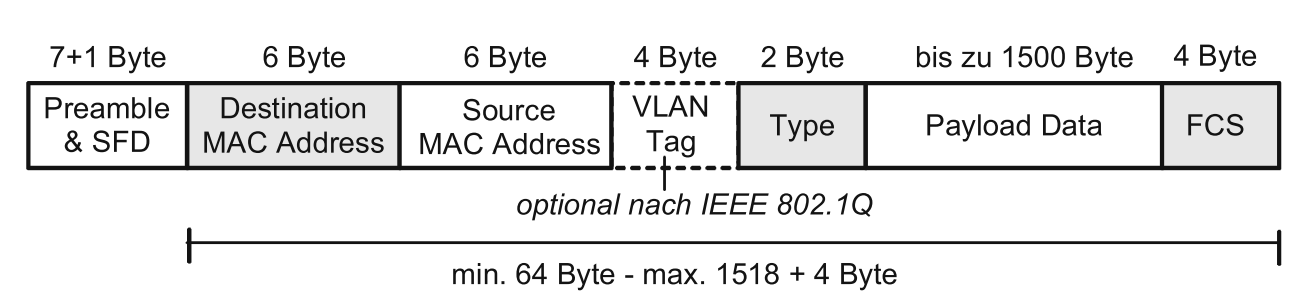
\includegraphics[width=\textwidth]{Zimmermann_EthernetPaket}
\label{fig:EthernetPaket}
\caption{Aufbau eines Ethernet-Pakets}
\quelle{\cite[140]{Zimmermann.2014}}
\end{figure}



\section{Schnittstellen}
Moderne Autos verfügen über eine Vielzahl von Schnittstellen, um eine Verbindung mit dem Fahrzeug herzustellen, sei es, um ein Multimediagerät zu verbinden oder zu Diagnosezwecken. Diese Schnittstellen können aber auch eventuell einem potentiellen Angreifer den Zugriff auf das Fahrzeugnetzwerk ermöglichen. Diese möglichen Angriffsvektoren können nach Checkoway et al \cite[1]{Checkoway.2011} in drei Kategorien eingeteilt werden. Diese drei Kategorien sind \glqq indirect physical access\grqq , \glqq short-range physical access\grqq{} und \glqq long-range physical access\grqq . Es folgt eine Beschreibung der Kategorien mit einer Übersicht der typischsten Schnittstellen eines modernen Autos.

\subsection{Indirect Physical Access}
Zu dieser Kategorie zählen sämtliche physische Schnittstellen, die direkt oder indirekt auf die internen Netzwerke des Autos zugreifen. Bei diesen Schnittstellen müsste ein Angreifer, um darauf zuzugreifen, mindestens einmalig physischen Zugang zum Fahrzeug haben oder über einen Vermittler arbeiten. 


\subsubsection{OBD-II Port} \label{OBD-II}
Der \ac{OBD}-II Port ist eine für Fachleute gedachte Schnittstelle auf den \acs{CAN}-Bus zu Diagnosezwecken.	Er befindet sich meist im Fußraum auf der Fahrerseite. Der Port umfasst 16 Pins, obwohl durch den Standard nur die Belegung von neun Pins vorgeschrieben ist. Die zusätzlichen Pins werden je nach Anbieter teilweise für den Zugriff auf zusätzliche Bussysteme verwendet. \cite[2]{Klinedinst.2016} \\
Üblicherweise wird an diesen Port ein Diagnosegerät des Herstellers oder einer Werkstatt angeschlossen. Das Diagnosegerät wird entweder von meist Windows-basierten Personal Computern programmiert oder fungieren als Mittler, um direkt mittels Laptop auf Port zuzugreifen \cite[3]{Checkoway.2011}. In beiden Fällen hat ein Windows-basierter PC direkt oder indirekt Zugriff auf das Netzwerk des Fahrzeugs. Der Hauptzweck dieses Gerätes ist es, Daten aus den \acsp{ECU} des Fahrzeugs zu sammeln. Das erfolgt über das Senden von diagnostischen \acs{CAN}-Paketen. Die betroffenen \acsp{ECU} senden anschließend die angefragten Daten. Diese Daten können dann beispielsweise zur Behandlung von Problemen verwendet werden.\\
Verbrauchermarktanbieter konnten allerdings die Kommunikationsarchitektur durch Reverse-Engineering verstehen und für andere Zwecke nutzen, zum Beispiel Pay-By-Mile-Versicherungen, Fahrzeuggebrauchstracking und kommerzielles Flottenmanagement \cite[3]{Klinedinst.2016}. \\

\subsubsection{Ladeanschluss eines Elektro-Autos}
Elektronische Fahrzeuge tanken nicht an Tankstellen wie ihre kraftstoffbetriebenen Pendants, sondern können an einer Steckdose oder speziellen, teilweise öffentlichen Ladestationen aufgeladen werden. Beim Ladevorgang an Ladestationen werden allerdings nicht nur elektrischer Strom sondern auch Daten ausgetauscht \cite[3]{Checkoway.2011}. Beispiele dafür können die Steuerung des Ladevorgangs, Authentifizierung und Autorisierung und Informationen über Ladezeit, Ladeleistung, Energieverbrauch und Batteriezustand sein. Dieser Datenaustausch ermöglicht einen effizienten und sicheren Ladevorgang, eine Abrechnung des bereitgestellten Stroms und eine Überwachung der Ladeinfrastruktur. Zudem können eine unautorisierte Nutzung der Ladestation oder eine Überlastung des Stromnetzes verhindert werden. 

\subsubsection{Entertainment}
Eine Vielzahl der physischen Schnittstellen eines Autos ist außerdem der Unterhaltung des Benutzers gewidmet. Beispielsweise bieten die meisten Autos mindestens einen USB- und einen Aux-Anschluss, damit Musik von externen Geräten abgespielt werden kann. Außerdem sind viele Autos mit einem CD-Laufwerk ausgestattet. Meist werden mehrere Audioformate unterstützt. Häufig sind die Entertainment-Systeme mit einem \acs{CAN}-Bus verbunden \cite[4]{Checkoway.2011}, um beispielsweise ganzheitliche Firmwareupdates zu ermöglichen. Außerdem kann das Infotainment-System Informationen von anderen Fahrzeugsystemen abrufen, um dem Fahrer relevante Daten anzuzeigen. Dazu gehören Informationen wie Fahrzeuggeschwindigkeit, Motordrehzahl oder Kraftstoffverbrauch, die dann auf dem Display angezeigt werden können.

\subsection{Short-Range Wireless Access}
Diese Kategorie umfasst Schnittstellen, deren Nutzung zwar drahtlos erfolgt, aber dennoch eine geringe physische Distanz zum Fahrzeug erfordert. Ein potenzieller Angreifer müsste sich für die Nutzung dieser Schnittstellen entweder in der Nähe befinden oder einen Transmitter in der Umgebung platzieren.


\subsubsection{Bluetooth}
Um Features wie eine Freisprecheinrichtung oder das Hören eigener Musik vom Smartphone zu realisieren, bieten die Infotainment-Systeme der meisten modernen Autos eine Bluetooth-Schnittstelle. Bluetooth ermöglicht die drahtlose Kommunikation zwischen dem Fahrzeug und externen Geräten wie Smartphones. Durch die Verbindung des Infotainment-Systems mit dem Controller Area Network des Fahrzeugs kann es mit anderen elektronischen Steuergeräten (\acsp{ECU}) kommunizieren. Diese Integration ermöglicht eine nahtlose Interaktion zwischen dem Infotainment-System und anderen Fahrzeugsystemen.
Die Bluetooth-Verbindung eröffnet Möglichkeiten für die Nutzung von verschiedenen Funktionen und Diensten. Eine der häufigsten Anwendungen ist die Freisprecheinrichtung, die es dem Fahrer ermöglicht, Anrufe über das Infotainment-System zu tätigen und entgegenzunehmen, ohne das Telefon in die Hand nehmen zu müssen. Das Infotainment-System wird über Bluetooth mit dem Telefon gekoppelt und kann auf die Telefonkontakte zugreifen, Anrufe initiieren und Anrufinformationen auf dem Display anzeigen.
Darüber hinaus ermöglicht die Bluetooth-Schnittstelle auch die drahtlose Übertragung von Audiodateien vom Smartphone zum Infotainment-System. Fahrer und Insassen können ihre eigenen Musikbibliotheken, Streaming-Dienste oder Podcasts über das Fahrzeuglautsprechersystem abspielen. Das Infotainment-System fungiert als Empfänger für das Audiosignal, das vom Smartphone gesendet wird.

\subsubsection{Remote Keyless Entry}
\ac{RKE} Systeme, auch als Funkfernbedienung oder Keyless-Entry-Systeme bekannt, sind Technologien, die es Fahrzeugbesitzern ermöglichen, ihr Fahrzeug aus der Ferne zu verriegeln und zu entriegeln, ohne einen physischen Schlüssel verwenden zu müssen. Diese Systeme bieten eine bequeme und sichere Möglichkeit, auf das Fahrzeug zuzugreifen.
Ein typisches RKE-System besteht aus zwei Hauptkomponenten: einem Funksender (Fernbedienung) und einem Empfänger, der im Fahrzeug eingebaut ist. Die Fernbedienung ist normalerweise eine kleine tragbare Vorrichtung, die über eine oder mehrere Tasten verfügt. Durch Betätigen der Tasten sendet die Fernbedienung ein verschlüsseltes Funksignal mit einer bestimmten Reichweite an den Empfänger im Fahrzeug.
Der Empfänger im Fahrzeug erkennt das Signal der Fernbedienung und interpretiert es. Wenn das empfangene Signal korrekt und authentifiziert ist, führt das RKE-System die gewünschte Aktion aus. Das kann das Entriegeln oder Verriegeln der Türen, das Aktivieren oder Deaktivieren der Diebstahlalarmanlage oder das Öffnen der Kofferraumklappe sein. In einigen Fahrzeugen können auch weitere Funktionen über die Fernbedienung gesteuert werden, wie das Starten des Motors oder das Ein- und Ausschalten der Fahrzeugbeleuchtung.\\
Des Weiteren sind viele moderne Automobile mit sogenannten Passive Keyless Entry and Start Systemen ausgestattet. Diese basieren auf einem bidirektionalen Challenge-Response-Schema. Das Auto sendet eine Challenge, woraufhin der Autoschlüssel mit einer kryptographischen Antwort (Response) reagiert. Bei einer gültigen Antwort werden die Türen entriegelt, das Alarmsystem deaktiviert und das Starten des Motors ermöglicht. Eine Benutzerinteraktion ist nicht notwendig, der Schlüssel muss sich lediglich in einem Umkreis von in der Regel etwa einem Meter zum Fahrzeug befinden. \cite[930]{Garcia.2016} \\
RKE-Systeme nutzen verschiedene drahtlose Kommunikationstechnologien wie Radiofrequenz (RF) oder Infrarot (IR), um die Signale zwischen der Fernbedienung und dem Fahrzeug zu übertragen \cite[4]{Checkoway.2011}. RF-basierte Systeme sind am weitesten verbreitet, da sie eine größere Reichweite bieten und nicht auf Sichtverbindung angewiesen sind.

\subsubsection{Reifendruck-Kontrollsystem}
Ein weiteres drahtloses Netzwerk in Fahrzeugen stellt das \ac{RDKS} oder auf englisch Tire Pressure Monitoring System (TPMS) dar. Die Integration eines solchen Systems ist in vielen Ländern gesetzlich vorgeschrieben. Neben der Vermeidung von Reifenpannen verspricht die Warnung vor unteraufgepumpten Reifen eine Steigerung der Verkehrssicherheit und Kraftstoffeffizienz, da der richtige Reifendruck die Traktion, den Bremsweg und den Rollwiderstand verbessert. Das Reifendrucküberwachungssystem misst kontinuierlich den Luftdruck in allen Reifen von Personenkraftwagen, Lastwagen und Mehrzweckfahrzeugen und warnt den Fahrer, wenn ein Reifen signifikant unteraufgepumpt ist. Es gibt sowohl direkte als auch indirekte Messverfahren. Bei einem direkten Messsystem werden batteriebetriebene Drucksensoren in jedem Reifen verwendet, um den Reifendruck zu messen, und die Daten werden über einen Funkfrequenz (RF)-Sender übertragen, da eine Verkabelung von einem rotierenden Reifen zur elektronischen Steuereinheit des Fahrzeugs schwierig umzusetzen ist. Die empfangende Reifendrucksteuereinheit analysiert die Daten und kann über das \ac{CAN} Ergebnisse oder Befehle an den zentralen Bordcomputer senden, um beispielsweise eine Warnmeldung auf dem Fahrzeugdashboard auszulösen. Indirekte Messsysteme leiten den Druckunterschied zwischen den Reifen aus den Unterschieden in der Rotationsgeschwindigkeit ab, die mithilfe der \ac{ABS}-Sensoren gemessen werden können. Ein Reifen mit niedrigerem Druck muss schneller rotieren, um die gleiche Strecke wie ein Reifen mit höherem Druck zurückzulegen. Die Nachteile dieses Verfahrens sind jedoch eine geringere Genauigkeit, die Kalibrierung durch den Fahrer und die Unfähigkeit, den gleichzeitigen Druckverlust in allen Reifen zu erkennen. Daher werden primär direkte Reifenkontrollsysteme verwendet. \cite[1]{Rouf.2010}

\subsubsection{Wireless LAN}
Viele Hersteller statten ihre modernen Autos heutzutage mit einer \ac{WLAN}-Schnittstelle aus \cite[4]{Checkoway.2011}. Die Technologie wird für verschiedene Anwendungsfälle eingesetzt. Viele moderne Autos sind mit Infotainment-Systemen ausgestattet, die WLAN verwenden, um eine drahtlose Verbindung zum Internet herzustellen. Dadurch können Insassen auf Streaming-Dienste, Musik, Online-Radio, und andere Online-Inhalte zugreifen. \acs{WLAN} ermöglicht auch Over-the-Air-Updates für das Infotainment-System, um Softwareaktualisierungen und neue Funktionen bereitzustellen. Auch für den Rest des Fahrzeugs lassen sich je nach Modell teilweise Softwareupdates über \acs{WLAN} herunterladen. Zum Beispiel die Autos von Tesla bieten dieses Feature. Darüber hinaus ermöglicht \acs{WLAN} den Passagieren im Auto in manchen Fahrzeugen die drahtlose Verbindung ihrer mobilen Geräte wie Smartphones, Tablets und Laptops mit dem Internet.
Schließlich werden \acs{WLAN}-basierte Standards in der Fahrzeug-zu-Fahrzeug-Kommunikation eingesetzt. Diese Art der Kommunikation wird auch Dedicated Short-Range Communications (DSRC) genannt \cite[4]{Checkoway.2011}. Durch den Datenaustausch zwischen Fahrzeugen sollen beispielsweise Kollisionen frühzeitig erkannt und verhindert werden. \\
Um die genannten Features umsetzen zu können, ist größtenteils eine Verbindung der \acs{ECU} mit der \acs{WLAN}-Schnittstelle zum Controller Area Network notwendig. Somit kann in vielen Fahrzeugen auch über \acs{WLAN} theoretisch indirekt auf den \acs{CAN}-Bus zugegriffen werden.



\subsection{Long-Range Wireless Access}
Zu dieser letzten Kategorie zählen alle Zugriffskanäle, die aus großer Entfernung, nämlich mehr als einem Kilometer, zugegriffen werden kann. Immer mehr Autos bieten auch derartige Schnittstellen. Diese lassen sich in zwei Kategorien einteilen: Broadcast Kanäle und Adressierbare Kanäle. \cite[4]{Checkoway.2011}

\subsubsection{Broadcast Kanäle}
Broadcast Kanäle sind Kanäle, die nicht speziell auf ein bestimmtes Fahrzeug ausgerichtet sind, sondern von Empfängern nach Bedarf empfangen werden können. Neben der externen Angriffsfläche können weitreichende Broadcastmedien als Steuerungskanäle attraktiv sein (z. B. zum Auslösen von Angriffen), da sie schwer zuzuordnen sind, mehrere Empfänger gleichzeitig steuern können und Angreifer keine genaue Adressierung ihrer Opfer benötigen.
Das moderne Automobil umfasst eine Vielzahl von Empfängern für weitreichende Signale: \ac{GPS}, Satellitenradio, Digitalradio und das Radio Data System (RDS) und der Traffic Message Channel (TMC), die als digitale Unterträger auf vorhandenen FM-Bändern übertragen werden. Die Reichweite solcher Signale hängt von der Sendeleistung, Modulation, Gelände und Störungen ab. Im Allgemeinen werden diese Kanäle in das Mediasystem eines Autos (Radio, CD-Player, Satellitenempfänger) implementiert, das, wie bereits erwähnt, häufig über interne Automobilnetzwerke Zugriff auf andere wichtige Automotive-ECUs ermöglicht. \cite[4\psq]{Checkoway.2011}

\subsubsection{Adressierbare Kanäle}
Über adressierbare Kanäle lassen sich individuelle Fahrzeuge direkt ansteuern. Die Verbindung erfolgt in der Regel über das Mobilfunknetz.\\
Durch diese Kanäle können viele Funktionen bereitgestellt werden. Dazu gehören die Unterstützung von Sicherheit (Unfallberichterstattung), Diagnose (frühzeitige Warnung bei mechanischen Problemen), Diebstahlschutz (Fernverfolgung und Deaktivierung) und Komfort (Zugriff auf Daten wie Fahrtrichtungen oder Wetterinformationen). \cite[5]{Checkoway.2011} \\
Da diese Kanäle meist eine hohe Bandbreite bieten, über große Distanzen und in beide Richtungen funktionieren und das direkte Ansteuern von individuellen Fahrzeugen ermöglichen, sind diese Schnittstellen für potenzielle Angreifer besonders interessant \cite[5]{Checkoway.2011}.


\section{Cyber Security}
\subsection{Security versus Safety}
Der deutsche Begriff \glqq Sicherheit\grqq{} ist mehrdeutig, was ihn für eine genaue, technische Definition ungeeignet macht. In der IT-Sicherheit wird zwischen den beiden englischen Begriffen \glqq Safety\grqq{} und \glqq Security\grqq{} unterschieden.
\subparagraph{Safety}
\glqq Der Begriff Safety bezeichnet die funktionale Sicherheit, bzw. die Betriebssicherheit eines Systems. Ein System darf seine Umgebung etwa durch undefiniertes, unzulässiges Verhalten oder Zustände nicht gefährden. Safety schützt somit Mensch und Umwelt vor negativen Einflüssen des Systems, etwa durch Fehlverhalten und Ausfälle.\grqq{} \cite[2]{Wurm.2022}
\subparagraph{Security}
\glqq Der Begriff Security bezeichnet die Informations- und Datensicherheit bzw. die Angriffssicherheit eines Systems. Security umfasst alle Eigenschaften und Maßnahmen, die das System vor absichtlichen und unabsichtlichen Bedrohungen
von außen schützen. Security schützt somit das System vor negativen Einflüssen von Mensch und Umwelt, wie etwa Bedrohungen und Angriffe. Während sich die sog. klassische IT-Security auf die Absicherung der informationstechnischen Systeme eines Unternehmens wie etwa Computer, Server, Netzwerke und Internetanbindungen konzentriert, zielt die Cybersecurity im Kontext des Automotive Bereichs auf die Absicherung deren Produkte ab.\grqq{} \cite[2\psq]{Wurm.2022}\\

Safety bezieht sich somit mehr auf die Sicherheit des Nutzers während sich die Security eines Systems mehr auf die Daten und das System an sich fokussiert.

\subsection{Security Lifecycle}
\cite{Wurm.2022}
\subsection{ISMS}


\chapter{Angriffsflächen}
\subsection{Bootvorgang}
\cite{Wurm.2022}

\subsection{Remote Keyless Entry}
\cite{Garcia.2016}


\chapter{Schutzmaßnahmen}
\subsection{SecureBoot}
\cite{Wurm.2022}[84]